\chapter{CCD-based Multispectral Frequency-Domain DOT of Breast Cancer}

\section{Introduction}


\section{Previous Breast Imaging Device}
Our breast imaging efforts have been focused on translating DOT techniques into the clinical setting. The previous clinical DOT device (Gen2)  has been successfully used in previous studies [CITATIONS] and we have been working to build on this success with improved capabilities in our current (Gen3) device. The primary upgrades in features are 1) frequency domain measurements in the transmission geometry using heterodyne measurement techniques, 2) addition of a profilometry system for enhanced breast segmentation for reconstruction, and 3) improved clinical patient interface. In this chapter, I will provide an overview of the new features and initial results.

\section{Previous Breast Imaging Device (Gen2)}
The Gen2 DOT imaging device [FIGURE] take data in the parallel-plate compression geometry. It measures multispectral continuous-wave (CW) measurements in the transmission geometry. In addition, it takes frequency-domain measurements in the remission geometry to determine bulk optical property values. The patient lies prone on a flat bed with her breast inserted inside a recessed box with a grid of fiber sources on one side (source plate) and a anti-reflection coated window on the other side (detector plate). The source plate is moved axially to softly compress the breast against the detector plate with the distance between the parallel plates varying from 5 to 7 cm. The box is filled with a matching fluid with optical properties similar to average human breast tissue. The matching fluid consists of water, india ink (for absorption) and intralipid (for scattering).

The source plate has 45 fiber positions arranged in a 9x5 square grid with a spacing of 1.6 cm between nearest neighbors. The sources are measured in series using cascading optical switches (DiCon Fiber Optics, Richmond, CA). At each source position six measurements are made at varying wavelengths (650, 690, 750, 785, 830, 905 nm) using fiber-coupled laser diodes. On the detection side, a CCD camera (Roper Scientific, Trenton, NJ, VersArray:1300F) collects the light that exits in the transmission geometry focused on the detection window. A image is obtained for for each source + laser combination with an exposure time of 500 ms. From each image a  A 24$\times$41 grid of 984  decimated set is selected from the CCD after 2x2 hardware binning of the pixels. For the frequency-domain remission measurements, four out of the six lasers are modulated at 70MHz. At these wavelengths measurements are made with additional grid of 3mm detector fibers arranged on the source plate in a 3x3 grid with 1.6 cm spacing. The light from these fibers are collected by an avalanche photodiode for homodyne frequency-domain measurements.


\section{Clinical Breast Imaging Device}
The core features that we wanted implemented for the device was to have a diffuse optical tomography device with multispectral and frequency-domain capabilities to improve quantification and separation of absorption and scattering in our image reconstruction. That the system was CCD based allow us to also collect a large number ($10^6$) of source detector pairs in parallel for improved resolution. In addition a supplimental pair of profilometry imaging system were designed and built (discussed later in the section) to provide 3 surface information about the breast shape to improve segmentation the 3D optical reconstruction of the breast.  Finally, significant effort was made to build a clinical grade device with a patient interface that maximized comfort and minimized movement during our measurement. Software for the device was also developed to enable simple and streamlined operation by our clinical collaborators.

The schematic for the clinical breast imaging prototype that I built is shown in Fig.~\ref{fig:Gen3schem}. The patient lies prone on a modified biopsy bed while one breast is centered and sagittally compressed between the source plate and window in the breast tank. Typical thickness of compression varies between 56mm and 70mm. The tank is filled with a solution of intralipid and india ink mixture to match the optical properties of tissue of the patient in the NIR wavelength range.

\subsection{Laser System}
The laser system schematic is shown in Fig.~\ref{fig:LaserSchem}. The imaging light source consists of five fiber pigtailed laser diodes with the wavelength of $660$, $690$, $785$, $808$, and $830\,{\rm nm}$ . These diodes are mounted on a custom copper block (Fig.~\ref{fig:LaserPic}) is driven and temperature controlled by a ILX mainframe with a module for each laser (instrument info). In addition, the lasers are amplitude modulated at $70\,{\rm MHz}$ using a frequency generator (Rhode and Schwartz, SMB100). RF signal from the frequency modulator is combined with the DC current from the ILX driver for each laser with ??? (minicircuit). The DC and RF voltage input for each laser was optimized using RF amplifiers, RF attenuators and adjusting the driver current for the best modulation depth ($>80 \%$) and sinusoidal waveform . The fiber from each laser is then coupled to a 6x1 100 $\mu m$ core optical switch (Optojenna) which allows the system to switch wavelengths in series.

\subsection{Source Position Switch and Source Plate}
The output fiber from the laser system is connected in series to a custom 1x210 channel optical galvo switch. Switching through 210 channels with a conventional cascade of switches used in the previous system based on mechanical or prism switch mechanisms is costly, slow, and have high throughput losses. The custom switch collimates light from a $100\,\mu{\rm m}$ input fiber and uses galvo controlled mirrors to direct the light into a fiber bundle with 210 $600\,\mu{\rm m}$ core fibers. Each fiber is connected to a custom hand-polished patch fiber with a metal ferrule tip that connects to the source plate. 209 of the source fibers are arranged in a 11x19 square grid with 8 mm spacing on each side on a black delrin plate. One of the remaining fiber is used as a calibration source placed far away from the source grid. The purpose of this calibration source will be discussed later in the chapter.

%\begin{figure}[t]
%\centering\includegraphics[width=7cm]{./figures/GalvoPic.png}
%\caption{\label{fig:GalvoSwitchPic}
%  Photograph of the (a) galvo switch and the (b) input face of the fiber bundle (c) custom patch cable (d) source plate
%\end{figure}

\subsection{Breast Tank and Patient Bed}
The breast imaging system is built around a modified biopsy bed. The bed allows for more of the breast to be inserted into the tank for greater breast coverage. The breast tank is located right below the hole. The tank consists a tank with a rail mounted source plate made out of black delrin. On the opposite side is an acrylic window with anti-reflective coating. The space between the window and the detection setup is covered by a light box that prevents stray signal from reaching the image intensifier and CCD.

%\begin{figure}[t]
%\centering\includegraphics[width=7cm]{./figures/BiopsyBedPic.png}
%\caption{\label{fig:BiopsyBedPic}
%  Photograph of the (a) galvo switch and the (b) input face of the fiber bundle
%\end{figure}

\subsection{Image Intensifier mounted CCD}
The detection system consists of a back-illuminated EMCCD (Andor iXon DV887, Ireland) with quantum efficiency optimized in the $500-700\,{\rm nm}$ range mounted with a gain-modulated image intensifier (Lambert Instruments, II8MD GENIII, Netherlands) with a P43 Phosphor screen with a peak emission at $545\, {\rm nm}$. The lens element in front of the image intensifier is a Xenon $25\,{\rm mm}$ $f/0.95$ C-Mount Lens for 1-Inch CCD (Schneider Optics, Germany). The $512 \times 512$ pixel CCD is cropped to a field of view of the breast tank window with a $2 \times 2$ hardware binning for an image $155 \times 200$ pixels with a dpixel of $0.33\, {\rm mm/pixel}$. The gain on the image intensifier is modulated at  $70\,{\rm MHz} + 1 {\rm Hz}$


\subsection{Frequency-Domain Heterodyne detection}
Our system uses the well known optical heterodyne detection scheme [cite] where the input signal $\omega_{s}$ is nonlinearly mixed with a reference signal at the same frequency which is offset by a small cross correlation frequency $\omega_{cc}$ such that $\omega_{g}=\omega_{s}+\omega_{cc}$ and the resulting beat frequency at $\omega_{cc}$ is measured.  In our system, $\omega_{s}$ and  $\omega_{g}$ are produced by a pair of phase-locked frequency generators the lasers are modulated at $70\,{\rm MHz}$ such that the light source intensity can be described as

\begin{equation}
I(t) = I_o + I_{\omega} cos(\omega_s t).
\end{equation}

Similarly, we modulate the gain of the image intensifier at $70\,{\rm MHz} + 1 {\rm Hz}$ so that the image intensifier sensitivity is

\begin{equation}
G(t) = G_o +GI_{\omega} cos({\omega_s+ t).
\end{equation}










\begin{equation}
I 
\end{equation}


\section{Profilometry}

\begin{figure}
\includegraphics[width = 1in]{./figures/4_Gen3/ProfilPic.jpg} 
\includegraphics[width = 3in]{./figures/4_Gen3/ProfilPic.jpg}\\
\includegraphics[width = 3in]{./figures/4_Gen3/ProfilPic.jpg}
\includegraphics[width = 3in]{./figures/4_Gen3/ProfilPic.jpg} 
\caption{testing}
\label{some example}
\end{figure}


\begin{figure}[htp]
\begin{center}
\includegraphics[width=5cm]{./figures/ProfilPic.jpg}
\caption{The slab case where the image method is used again to find  the solution. This time since there are two boundaries, we have to sum over a larger number of source and sink images.}
\label{slab}
\end{center}
\end{figure}


\section{Device characterization and testing}

\section{Clinical Results}